\graphicspath{{content/appendices/figures}}
\chapter{Extra Evaluation}
\label{appendix:extra_evaluation}

\section{Subjective Evaluation}
\label{sec:subjective_evaluation}


\section{Comparison with Pre-trained Models}
\label{sec:pretrained_comparison}

The results in Table~\ref{tab:ml_denoise} clearly show ConvTasNet as our highest-performing model. Importantly, all models in this project were trained entirely from scratch on our chosen dataset and adapted from literature to work with spectrogram-domain data. While this approach yielded strong results, it also means that these models are inherently specialized to the data they were trained on, and may not generalisewell to unseen or real-world audio conditions.

This underscores the value of pre-trained models in the field of speech enhancement. Pre-trained systems like \textit{Demucs}, \textit{VoiceFixer}, and \textit{DeepFilterNet} are designed to work across a wider range of audio conditions, having been trained on large and diverse datasets. They leverage transfer learning to adapt to new tasks or domains, which can be particularly beneficial when the target dataset is limited in size or diversity. These models are often built on architectures that have been shown to be effective and incorporate advanced techniques.

To contextualise the performance of our best model ConvTasNet. We compared it against these pre-trained systems, which are also designed for speech enhancement tasks. We used the same evaluation metrics as in our previous experiments and to ensure a fair comparison two samples are used for this single denoising task. The first sample is drawn from our native dataset, while the second is taken from the NOIZEUS~\cite{hu2007subjective}, a foreign benchmark dataset for speech enhancement research. This allows us to evaluate the generalization capabilities of these models across different datasets.

\vspace{1em}
\begin{table}[H]
\centering
\caption{Evaluation of Pre-trained Models vs ConvTasNet (per sample)}
\label{tab:pretrained_eval}
\begin{tabular}{|l|l|c|c|c|c|c|}
\hline
\textbf{Sample} & \textbf{Model} & \textbf{↑SNR} & \textbf{↓MSE} & \textbf{↓LSD} & \textbf{↑PESQ} & \textbf{↑STOI} \\
\hline
p232\_334 & ConvTasNet      & 12.40 & 0.0002 & 0.471 & 2.85 & 0.993 \\
p232\_334 & Demucs          & -2.95 & 0.0093 & 0.928 & 1.21 & 0.099 \\
p232\_334 & VoiceFix        & -2.26 & 0.0079 & 0.966 & 1.19 & 0.009 \\
p232\_334 & DeepFilterNet   & 21.62 & 0.0000 & 0.460 & 3.56 & 0.992 \\
\hline
sp07      & ConvTasNet      & -5.85 & 0.0059 & 1.614 & 1.04 & 0.230 \\
sp07      & Demucs          & -4.95 & 0.0048 & 1.378 & 1.04 & 0.243 \\
sp07      & VoiceFix        & -7.37 & 0.0084 & 1.565 & 1.04 & 0.193 \\
sp07      & DeepFilterNet   & 4.25  & 0.0006 & 1.012 & 1.34 & 0.848 \\
\hline
\end{tabular}
\end{table}


The results in Table~\ref{tab:pretrained_eval} offer important insights into the generalization capabilities of our trained from scratch ConvTasNet model compared to large scale Pre-trained models.

For the \texttt{p232\_334} sample from our native dataset, ConvTasNet performs exceptionally well, achieving strong scores across all metrics. An SNR of 12.40 dB, PESQ of 2.85, and a near perfect STOI of 0.993. This confirms the model’s robustness when applied to data similar to its training distribution. Interestingly, DeepFilterNet significantly outperforms ConvTasNet in SNR (21.62 dB) and PESQ (3.56), suggesting that either a superior architecture or a more advanced training strategy may have been used to achieve such state of the art results. It is unclear, however, whether DeepFilterNet had prior exposure to this dataset or whether the sample is also foreign to its training distribution.

In contrast, Demucs and VoiceFixer underperform on this native sample, negative SNR values and extremely low intelligibility scores (STOI < 0.1). This suggests a mismatch between their design assumptions and the characteristics of our spectrogram domain dataset, or possibly issues in the integration process used to integrate these models into our evaluation pipeline.

The results shift significantly for the \texttt{sp07} sample from the NOIZEUS dataset~\cite{hu2007subjective}. Here, ConvTasNet's performance deteriorates, yielding a negative SNR of -5.85 dB and a PESQ of 1.04. This decline is expected given the differences in microphone quality, noise types, and recording environments. All of which presented unseen conditions for our model. Similar trends are observed for Demucs and VoiceFixer, both of which also produce negative SNRs and generally lower perceptual scores. However, ConvTasNet still slightly outperforms them in perceptual metrics, suggesting a marginally better generalization capacity.

DeepFilterNet again shows the strongest generalization, maintaining a positive SNR of 4.25 dB and a PESQ of 1.34. Although this performance is lower than its results on our native sample, it remains superior to all other models. This indicates more robust generalisation to foreign audio. This also suggests that the \texttt{sp07} file may be a particularly challenging test case due to its distinct noise profile and recording setup.

Overall, these results validate both the strengths and limitations of our trained from scratch models. ConvTasNet performs strongly within its domain but struggles with generalization. Highlighting the challenge of deploying domain specific models in uncontrolled environments. Conversely, Pre-trained models particularly DeepFilterNet, demonstrate better cross-domain resilience. This underscores the value of large scale, diverse training data and advanced model design when targeting real-world deployment.

\begin{figure}[H]
\centering
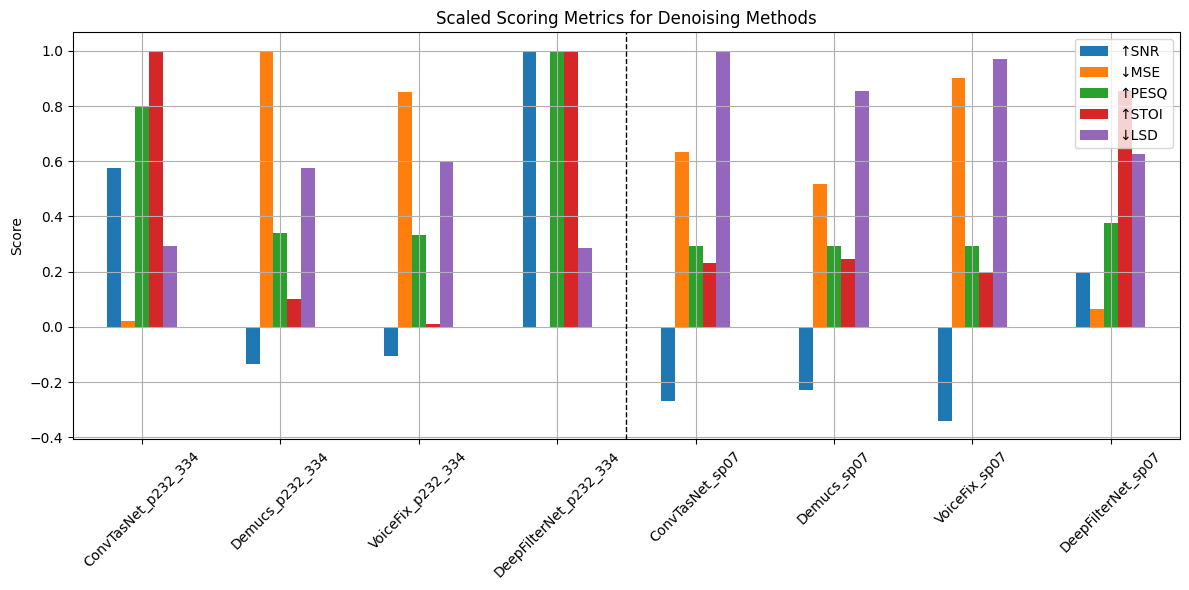
\includegraphics[width=1\textwidth]{pre_trained_metrics.png}
\caption{Scaled Scoring of ConvTasNet vs Pre-trained Models}
\label{fig:pretrained_metrics}
\end{figure}
\noindent

Figure~\ref{fig:pretrained_metrics} provides a visual representation of the evaluation metrics for both ConvTasNet and the Pre-trained models. The scores are normalized to facilitate better visual comparison.

